% TODO:
% - compare final results with novel environment (different way-points)
% - textit vs emph vs mathit


\section{Introduction}


% (1) Introductory paragraph: Very briefly: What is the problem and why is it relevant to the audience attending *THIS CONFERENCE*? Moreover, why is the problem hard, and what is your solution? You must be brief here. This forces you to boil down your contribution to its bare essence and communicate it directly.
Autonomous unmanned ground vehicles (UGV) provide an excellent solution to tasks that require searching or monitoring in environments deemed too remote or dangerous for humans.
%
Consider \emph{search and rescue}: after a natural disaster a UGV can be used by first responders to help locate victims in unstable and hazardous locations.
%
% Compared with an unmanned aerial vehicle (UAV), a
UGVs have long operating durations, can carry heavy payloads (\eg{}, sensors), and can search in narrow and covered places such as forests and caves.
%
% Ideally, a heterogeneous swarm of UAVs and UGVs would coordinate to gain the advantages of both search modes~\citep{Kruijff.SearchAndRescue.ICFSR.2014}.
%
% In this paper, however, we limit our investigation to UGVs.
% In particular, we show results for improving the mobility of Adabot, a UGV that includes wheel struts.


% (2) Background paragraph: Elaborate on why the problem is hard, critically examining prior work, trying to tease out one or two central shortcomings that your solution overcomes.
% One issue that arises during the design of a UGV is how to ensure that the system
Ensuring that a UGV can handle many different types of terrain is an ongoing challenge.
%
Researchers have invented several different methods for addressing the issue of mobility in varied terrain.
%
Specifically, robots have been designed with
treaded wheels,
tracks,
legs~\citep{Haldane.ICRA.VelociRoACH.2013},
legged-wheels (wheels are rimless, wheel spokes make contact with the ground)~\citep{Saranli.IntJrnRoboRes.RHex.2001,Quinn.IROS.Whegs.2002,Eich.SSRR.Stair-climb-SAR.2008,Kenneally.IEEERobAutLetters.Legged-robots.2016},
wheeled-legs (wheels are on the end of legs and the suspension is potentially actively actuated)~\citep{Grand.2004.IJRR.StabilityTractionOptimization,Zheng.2015.AME.DesignAnalysisWheellegged,Smith.IROS.Tri-wheel.2015}, and
transformable wheels~\citep{Kim.2014.ITR.WheelTransformerWheelLeg,Chen.2014.ITM.QuattropedLegWheel,Chen.2017.ITR.TurboQuadNovelLeg,Wei.2017.JMR.DesignImplementationLeg}.
%
Although these systems provide an advantage over traditional wheeled robots, optimization is not performed in the vast majority of these studies.
%
Moreover, as identified by \citet{Mintchev.2016.IRAM.AdaptiveMorphologyDesign}, most researchers in the area of transformable wheels currently focus on the mechanical design and leave control and decision making to future work.
%
For example, most robots with transformable wheels are controlled remotely~\citep{She.IROS.Transformable-wheel.2015,Chen.2017.ITR.TurboQuadNovelLeg}, and \citet{Kim.2014.ITR.WheelTransformerWheelLeg} designed a passive triggering mechanism that does not require any controller input.
% \blue{How could EA help?}


% (3) Transition paragraph: What keen insight did you apply to overcome the shortcomings of other approaches? Structure this paragraph like a syllogism: Whereas P and P => Q, infer Q.
The device in this study, the \emph{Adabot} (see \figref{fig:adabot}), includes transformable wheels that can smoothly be converted from a round wheel, to a wheel with tire \emph{studs}, to a legged-wheel.
%
Wheel transformations are performed by extending wheel struts radially outward from the center of the wheel (see \figref{fig:wheel-extender}).
 % (see \secref{sec:adabot} for details \ref{sec:adabot} \nameref{sec:adabot}).
%
Adabot has been optimized using an evolutionary algorithm such that its physical characteristics and its controller are better able to handle terrain that includes obstacles of varying sizes.
%
In previous work~\citep{Clark.2017.SSCI.Adabot}, a similar system was optimized to maximum forward velocity over uneven terrain.
%
The present study differs in two main ways: (1) here we evolve controllers for a more difficult task: \emph{way-point following}, and (2) we analyze results from evolving two controller types of feedback controllers (rather than feed-forward).



% (4) Details paragraph: What technical challenges did you have to overcome and what kinds of validation did you perform?
In this study, we evolve the robot's chassis dimensions, its wheel radius, the number of wheel struts,
% (described in \secref{sec:adabot}),
along with either a finite state machine (FSM) controller or an artificial neural network (ANN) controller.
%
The best evolved FSMs and ANNs are analyzed and compared.
%
For this initial work, to ensure that we are able to effectively analyze the ANN, the network only has three input nodes, zero hidden nodes, and three output nodes. The inputs are fully connected to the outputs.
%
The network is only slightly more complex than a Type 2 Braitenberg vehicle~\citep{Braitenberg.Vehicles.Book.1986}.
%
Conclusions drawn from our analysis are used to create a set of design principles for a new controller that takes advantage of both techniques.
%
In particular, it is attractive to design a controller that is not a black-box like an ANN but less rigidly defined than an FSM.
%
% \blue{hybrid controller}
%
%
% (5) Assessment paragraph: Assess your results and briefly state the broadly interesting conclusions that these results support. This may only take a couple of sentences. I usually then follow these sentences by an optional overview of the structure of the paper with interleaved section callouts.
% The results presented in this study demonstrate how a UGV can be optimized to improve robustness.
%
% Specifically, evolving Adabot has made it more robust in the presence of varied terrain.
%
% The techniques and concepts presented in this study can be applied to the optimization of any physical system.
%
Source code has been made available on GitHub\footnote{\url{https://github.com/anthonyjclark/adabot02-ann}}.

% %\vspace{-0.1in}

\begin{figure}[!ht]
    \centering

    % \subfloat[]{\fbox{\crule[white]{0.4\columnwidth}{2cm}}}
    % \hfil
    % \subfloat[]{\fbox{\crule[white]{0.4\columnwidth}{2cm}}}

    \subfloat[Simulated Device]{%
        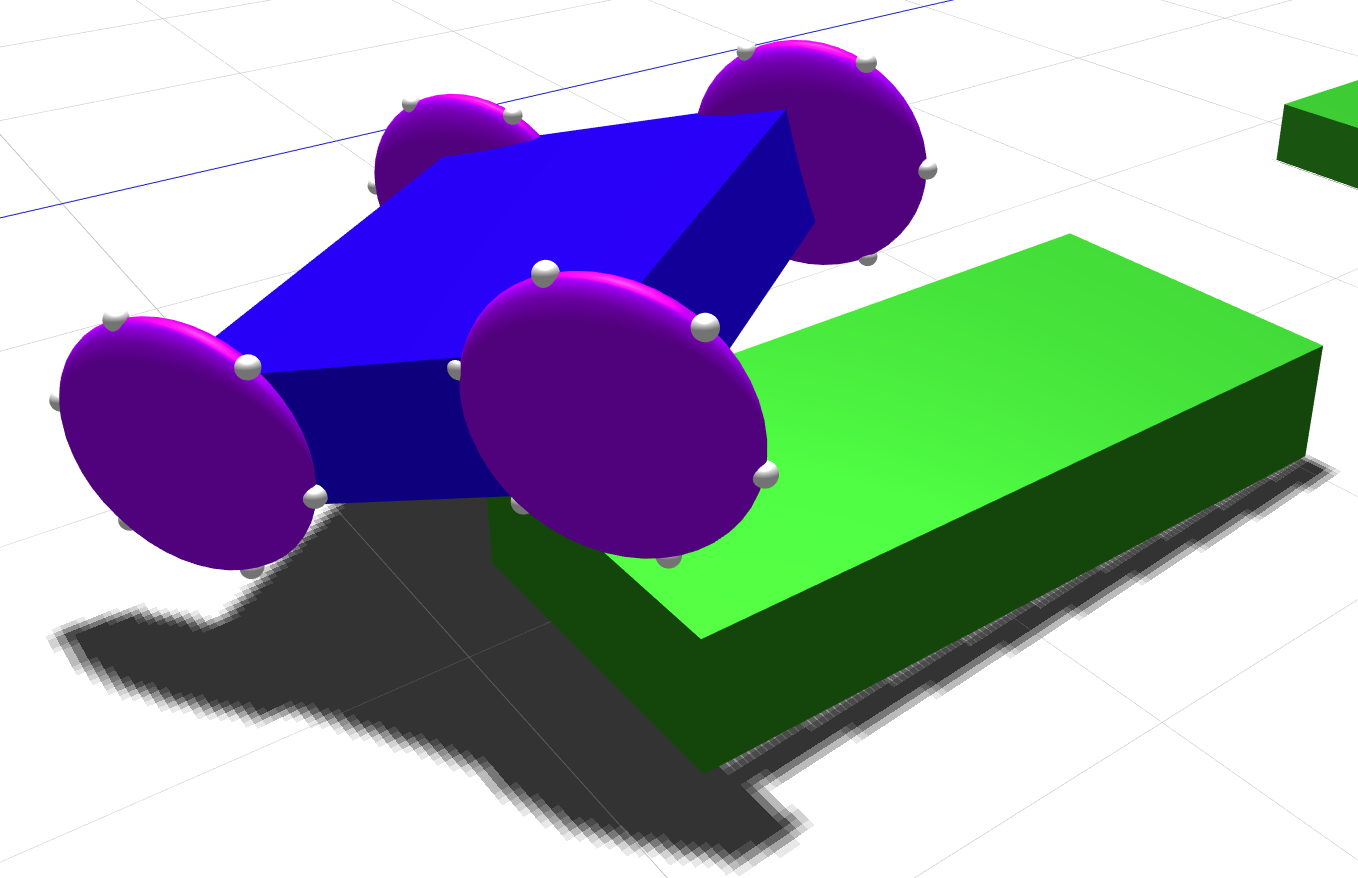
\includegraphics[width=0.4\textwidth,valign=c]{figures/1-introduction/simulation-climbing.png}%
        \vphantom{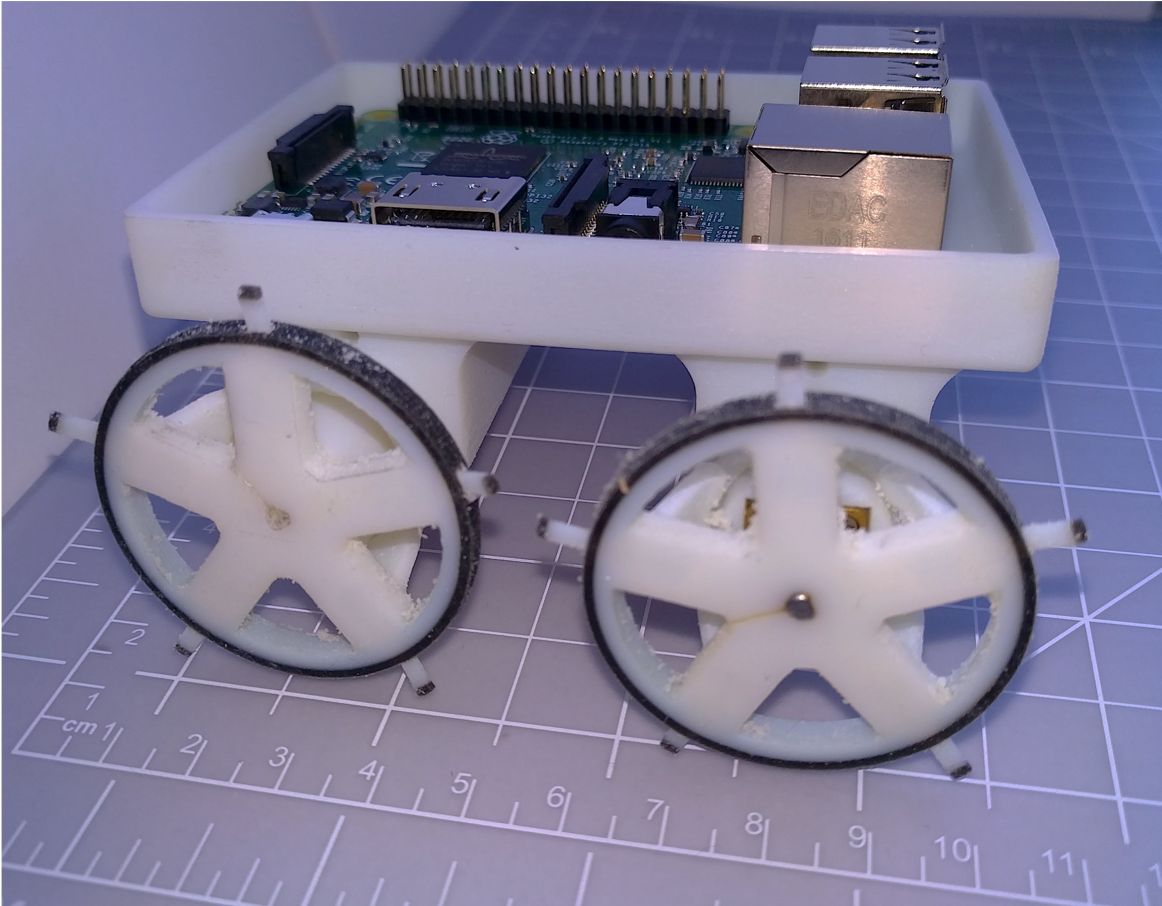
\includegraphics[width=0.4\textwidth,valign=c]{figures/1-introduction/perspective-image.jpg}}%
    }\quad
    \subfloat[3D Printed Prototype]{%
        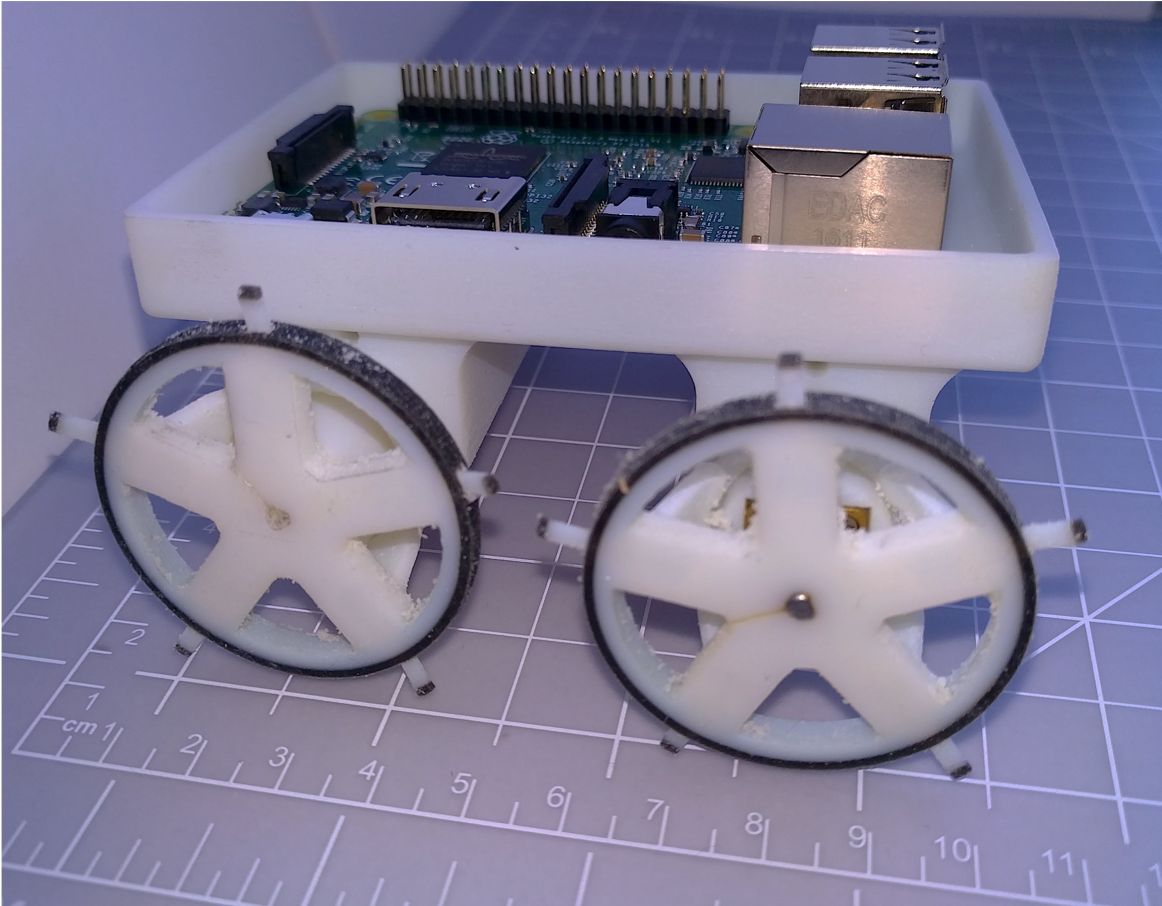
\includegraphics[width=0.4\textwidth,valign=c]{figures/1-introduction/perspective-image.jpg}%
    }

    %\vspace{-0.05in}

    \caption{Adabot, a UGV with transformable wheels.}
    \label{fig:adabot}

    %\vspace{-0.15in}

\end{figure}

% %\vspace{-0.1in}
